\documentclass[
12pt, % 字体大小
a4paper, 
oneside, % 单面打印(双面为twoside)
headinclude,footinclude, % 页眉页脚包含在文本区域内,确保不被裁剪或掩盖
]{scrartcl}
% 主题和样式
\usepackage[
nochapters, % 无章节层级 
beramono, % 等宽字体样式
eulermath, % 数学公式Euler字体
pdfspacing, % 字间距
dottedtoc % 点线式目录
]{classicthesis}
\usepackage{arsclassica} 
%----------------------------------------------------------------------------------------
% 输入和页面排版
\usepackage[T1]{fontenc} % 字体编码
\usepackage[utf8]{inputenc} % 输入编码
\usepackage{ctex} % 汉语
\usepackage{amsmath,amssymb,amsthm} % 数学公式
\usepackage{indentfirst} % 缩进
\setlength{\parindent}{2em} % 段落缩进
\usepackage[
top=2cm,
bottom=2cm, 
left=2cm,
right=2cm, 
headheight=20pt, 
includeheadfoot 
]{geometry} % 页面
\usepackage{scrlayer-scrpage} % 页眉页脚
\renewcommand{\sectionmark}[1]{\markright{\spacedlowsmallcaps{#1}}}
\renewcommand{\subsectionmark}[1]{\markright{\thesubsection~#1}}
\lehead{\mbox{\llap{\small\thepage\kern1em\color{halfgray} \vline}\color{halfgray}\hspace{0.5em}\rightmark\hfil}} % 标题旁边标记页码
\cfoot{\hyperlink{toc}{\color{RoyalBlue}返回目录}} % 页脚返回目录链接
\pagestyle{scrheadings}
%----------------------------------------------------------------------------------------
% 图表和引用
\usepackage{graphicx} % 图像
\graphicspath{{Figures/}} % 图像路径
\usepackage{subfig} % 图组
\usepackage{float} % 浮动
\usepackage{enumitem} % 列表
\usepackage{varioref} % 交叉引用
%----------------------------------------------------------------------------------------
% 代码
\usepackage{listings}
\lstset{
    language=Matlab,
    basicstyle=\ttfamily\small,   % 字体
    numbers=left,                 % 行号
    numberstyle=\tiny\color{gray},
    stepnumber=5,
    numbersep=5pt,
    backgroundcolor=\color{white},% 背景
    tabsize=2,                    % 制表符宽度
    frame=single,                 % 边框
    captionpos=t,                 % 标题
    title=\lstname,
    breaklines=true,              % 换行
    breakatwhitespace=true,
    escapeinside={`}{`},          % 转义(中文注释)
}
\lstset{
    language=Python,            
    basicstyle=\ttfamily\small,   % 字体
    numbers=left,                 % 行号
    numberstyle=\tiny\color{gray}, 
    stepnumber=5,             
    numbersep=5pt,            
    backgroundcolor=\color{white},% 背景
    tabsize=4,                    % 制表符宽度            
    frame=single,                 % 边框
    captionpos=t,                 % 标题
    title=\lstname, 
    breaklines=true,              % 换行
    breakatwhitespace=false,   
    escapeinside={`}{`},          % 转义(中文注释)
}
\usepackage{algorithm} % 算法
\usepackage{algpseudocode}
\usepackage{mdframed} % 跨页框架
% 不浮动算法环境
\newcounter{myalgorithm}
\renewcommand{\themyalgorithm}{\arabic{myalgorithm}}
\newenvironment{myalgorithm}[1][]{
  \refstepcounter{myalgorithm}
  \begin{mdframed}[
    skipabove=\topskip,
    skipbelow=\topskip,
    needspace=3\baselineskip,
    linewidth=0.4pt,
    frametitlefont=\normalfont\bfseries,
    frametitle={算法 \themyalgorithm\if\relax\detokenize{#1}\relax\else:#1\fi},
    frametitlerule=true,
    frametitlerulewidth=0.4pt,
    repeatframetitle=true
  ]
  \begin{algorithmic}[1]
  \ifx\relax\detokenize{#1}\relax
    \addcontentsline{alg}{algorithms}{\makebox[7em][l]{算法~\themyalgorithm} }
  \else
    \addcontentsline{alg}{algorithms}{\makebox[7em][l]{算法~\themyalgorithm} #1}
  \fi
}{
  \end{algorithmic}
  \end{mdframed}
}
% 关键词
\algrenewcommand{\algorithmicwhile}{当}
\algrenewcommand{\algorithmicdo}{执行}
\algrenewcommand{\algorithmicend}{结束}
\algrenewcommand{\algorithmicif}{如果}
\algrenewcommand{\algorithmicthen}{那么}
\algrenewcommand{\algorithmicelse}{否则}
\algrenewcommand{\algorithmicfor}{对于}
\algrenewcommand{\algorithmicrepeat}{循环}
\algrenewcommand{\algorithmicuntil}{直到}
\algrenewcommand{\algorithmicloop}{循环}
\algnotext{EndFor}
\algnotext{EndIf}
\algnotext{EndLoop}
\algnotext{EndWhile}
%----------------------------------------------------------------------------------------
% 超链接与PDF信息
\usepackage{hyperref} 
\hypersetup{
colorlinks=true, % 彩色
breaklinks=true, % 断行
urlcolor=webbrown, % URL棕色
linkcolor=RoyalBlue, % 内部链接蓝色
citecolor=webgreen, % 引用绿色
bookmarks=true, % 书签
bookmarksnumbered,
pdftitle={}, 
pdfauthor={},
pdfsubject={}, 
pdfkeywords={}, 
pdfcreator={pdfLaTeX}, 
pdfproducer={LaTeX with hyperref and ClassicThesis} 
}
%----------------------------------------------------------------------------------------
% 目录与标题
\usepackage{titlesec} 
\AtBeginDocument{
    \renewcommand{\contentsname}{目\hspace{1em}录}
    \renewcommand{\listfigurename}{图\hspace{1em}片}
    \renewcommand{\listtablename}{表\hspace{1em}格}
    \renewcommand{\figurename}{图}
    \renewcommand{\tablename}{表}
    \setcounter{tocdepth}{3} % 目录深度
}
\theoremstyle{definition} 
\newtheorem{definition}{定义}
\theoremstyle{plain} 
\newtheorem{theorem}{定理}
\theoremstyle{remark}
\newtheorem{remark}{备注}
\newtheorem{example}{样例}
\usepackage{tocloft} % 目录
% 要点目录
\newlistof{tips}{tip}{要\hspace{1em}点}
\newcommand{\tip}[1]{
  \refstepcounter{tips}
  \textsuperscript{\textcolor{orange}{\textbf{\thetips}}}
  \addcontentsline{tip}{tips}{\makebox[7em][l]{要点~\thetips} #1}
}
% 算法目录
\newlistof{algorithms}{alg}{算\hspace{1em}法} 
\hyphenation{Fortran hy-phen-ation} % 单词断字规则
%----------------------------------------------------------------------------------------
% 题目和作者
\title{\normalfont\spacedallcaps{智能工程}} 
\date{}
%----------------------------------------------------------------------------------------
% 开始和目录
\begin{document}
\maketitle
\newpage
\tableofcontents 
\newpage
\listoffigures
\listoftables
\listoftips
\newpage
%----------------------------------------------------------------------------------------
\section{基础知识}
%------------------------------------------------
\paragraph{课程内容}
\begin{figure}[H]
\centering
\subfloat[课程内容]{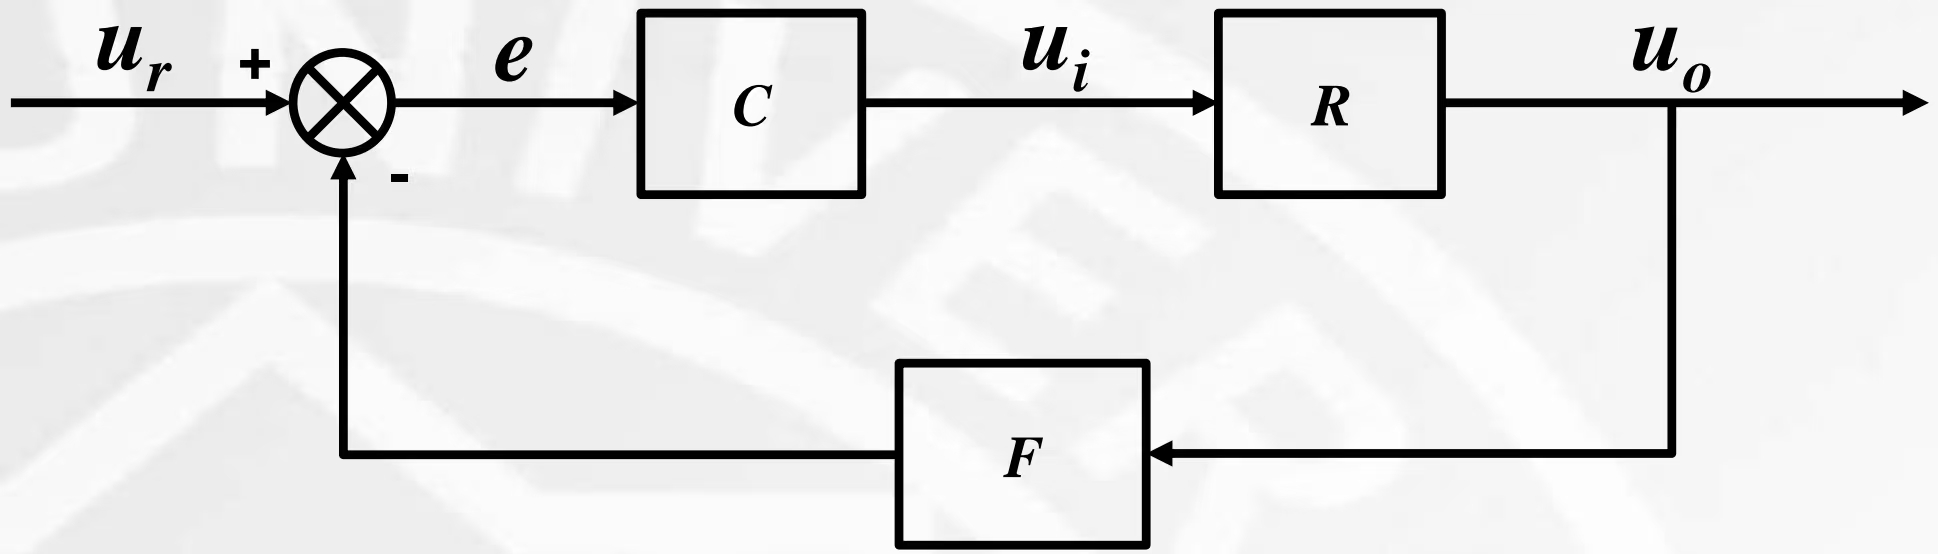
\includegraphics[width=.45\textwidth]{control}} \quad
\subfloat[工作流程]{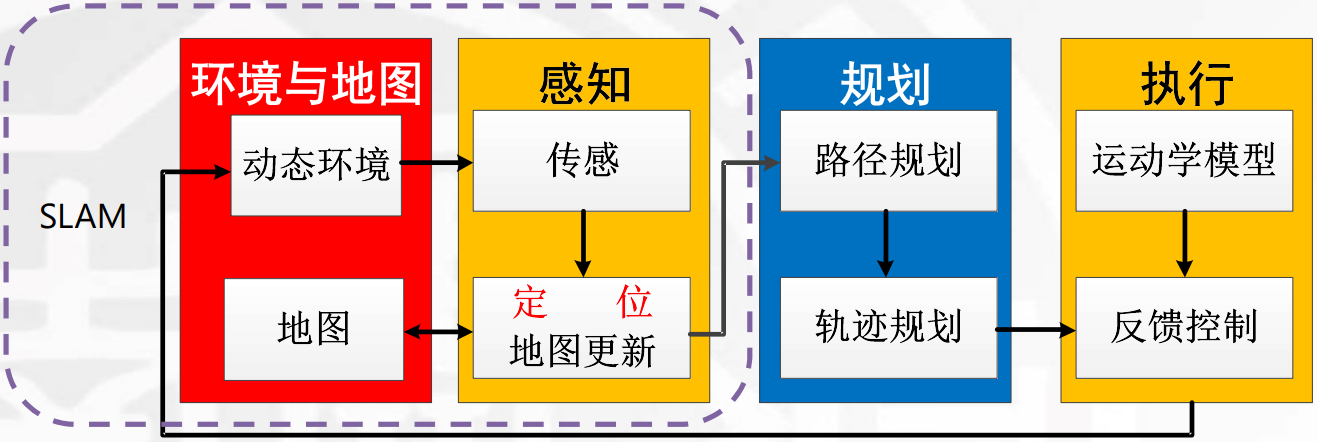
\includegraphics[width=.45\textwidth]{workflow}}
\caption[课程内容]{课程内容}
\end{figure}

\begin{table}[hbt]
\caption{课程内容}
\centering
\begin{tabular}{|p{0.5cm}|p{2cm}|p{2cm}|p{2cm}|p{2cm}|p{2cm}|p{2cm}|p{2cm}|}
\hline
& $ u_i $ & $ u_o $ & $ R $ & $ F $ & $ u_r $ & $ e $ & $ C $ \\
\hline
概念 & 系统输入 & 系统输出 & 系统模型 & 反馈单元 & 系统给定 & 系统误差 & 控制器 \\
\hline
含义 & 能对被控对象施加作用的手段 & 作业目标相应的可测系统状态 & 系统输入输出映射 & 系统输出映射变换 & 系统作业目标 & 作业目标与系统当前测量状态差值 & 系统误差与输入映射 \\
\hline
内容 & \multicolumn{3}{c|}{机器人运动学} & \multicolumn{2}{c|}{机器人控制} & 机器人感知 & 机器人轨迹规划 \\
\hline
\end{tabular}
\end{table}
%------------------------------------------------
\paragraph{课程案例}\label{sec:two_wheel}
移动机器人->轮式机器人->两轮差速机器人。
\begin{figure}[H]
\centering 
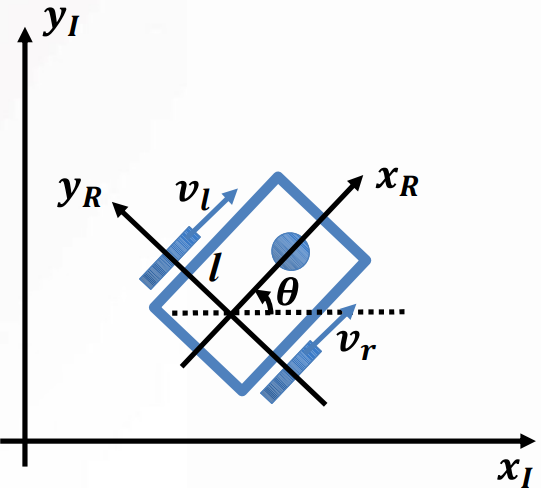
\includegraphics[width=0.4\textwidth]{two_wheel} 
\caption[两轮差速机器人模型]{两轮差速机器人模型}
\end{figure}
\begin{itemize}
\item 车轮半径$ r $。
\item 两轮转速$ \varphi_l,\varphi_r $:$ v_i = \varphi_i r $。
\item 车轮到两轮中间点距离$ l $。
\end{itemize}

\begin{enumerate}
\item 求正运动学模型\ref{sec:example1}。
\end{enumerate}
%------------------------------------------------
\section{机器人运动形态}
%------------------------------------------------
\subsection{移动机器人}
%------------------------------------------------
\paragraph{自然界运动形态特点}
\begin{itemize}
\item 能量利用率高。
\item 适应野外复杂环境。
\item 与身体尺寸、结构相适应。
\item 运行速度高。
\end{itemize}
%------------------------------------------------
\paragraph{机器人实现自然界运动形态问题}
\begin{itemize}
\item 机械结构、能量密度、感知与控制决策能力困难。
\item 安全性、可靠性差。
\item 成本高。
\item 于人造环境低效。
\end{itemize}
%------------------------------------------------
\paragraph{运动(Locomoion)}
机器人与环境的物理交互方式。
\begin{itemize}
\item 稳定性。
\item 接触特性。
\item 环境特性。
\end{itemize}
%------------------------------------------------
\subsection{腿式机器人}
%------------------------------------------------
\subsubsection{腿式机器人}
%------------------------------------------------
\paragraph{研究意义}
\begin{itemize}
\item 复杂恶劣环境的高适应性。
\item 点接触的高通过能力。
\item 高实现难度:系统控制多自由度,实时感知环境。
\end{itemize}
%------------------------------------------------
\paragraph{腿数影响}
\begin{itemize}
\item 机构复杂度。
\item 控制复杂度。
\item 环境适应性:腿越多,通过性越好,环境适应性越强。
\item 系统稳定性\tip{腿式机器人稳定性}:腿数增加,由动态稳定向静态稳定过度。
\begin{itemize}
\item 动态稳定:执行器停止工作摔倒。运动过程中通常半数腿离地。
\item 静态稳定:执行器停止工作不摔倒。点接触需保证三腿同时着地,面接触需保证一条腿着地。
\end{itemize}
\end{itemize}
%------------------------------------------------
\paragraph{运动规划}
\begin{itemize}
\item 运动学分析。
\item 动力学分析。
\end{itemize}
%------------------------------------------------
\paragraph{步态}\tip{腿式机器人步态}
一个行进周期内各腿抬落组合,$ k $腿机器人的步态模式数量为$ N = (2^k - 1)! $。
%------------------------------------------------
\paragraph{单位距离能耗(COT)}
$ cot = \frac{\text{消耗能量}}{\text{重量} \times \text{运行距离}} $。
%------------------------------------------------
\subsubsection{四足机器人}
\begin{itemize}
\item 点接触:每条腿至少需要两个自由度,执行器较少,没有冗余。
\item 行走(静态平衡):一次移动一条腿,剩下腿支持身体,重心落在支持多边形内。适合攀爬,速度低,能效低。
\item 奔跑(动态平衡):一次移动多条腿,平衡建立在周期运动上。速度高,能效高,需要实时控制与执行。
\end{itemize}
%------------------------------------------------
\subsubsection{双足机器人}
%------------------------------------------------
\paragraph{两种方案}
\begin{itemize}
\item 静态稳定(日本):面接触,重心左右变换,速度低,环境适应性差,能效低。
\item 动态稳定(美国):点接触,重心适时调整,速度高,环境适应性强,能效高。
\end{itemize}
%------------------------------------------------
\paragraph{动态稳定运动机理}\tip{双足机器人运动机理}
\begin{itemize}
\item 倒立摆模型:类似纯滚动,步距越小越趋于圆。步态不自然,重心变化(需做功),落地冲击大。
\item 无源动态行走:摆动与向前摔落结合,势能转化为动能。
\item 弹簧负载倒立摆(SLIP):仿照动物腿肌肉,增加弹簧来缓冲并储存能量,运动具有对称性。其周期往复运动的动态稳定性可由庞加莱变换线性化后验证,条件为$ \lambda < 1 $(见PPT.2.34-43)。
\item 串联弹性驱动(SEA):更为高效,更符合生物的自然属性,基于运动学的位置控制,基于动力学的力矩控制。可由其获得稳定平台(见PPT.2.48-50)。
\end{itemize}
%------------------------------------------------
\subsection{轮式机器人}
%------------------------------------------------
\paragraph{研究意义}
\begin{itemize}
\item 人造环境下的高效性:滚动摩擦,无重心起伏。
\item 结构简单,可靠性高,成本低。
\item 控制简单,系统复杂度低。
\end{itemize}
%------------------------------------------------
\paragraph{轮数对稳定性的影响}
轮数增加,由动态稳定向静态稳定过度。
\begin{itemize}
\item 动态稳定:执行器停止工作摔倒。倒立摆模型。    
\item 静态稳定:执行器停止工作不摔倒。陀螺效应,随动轮效应。
\end{itemize}
%----------------------------------------------------------------------------------------
\section{机器人运动学}
%------------------------------------------------
\subsection{运动学模型}
表征机器人驱动(输入)和机器人空间位姿(输出)关系。

机械臂运动学模型与移动机器人运动学模型的区别:
\begin{itemize}
\item 机械臂本体坐标系固定,精度高;移动机器人本体坐标系随动,精度低。
\item 非完整约束\tip{非完整约束}:移动机器人只知道码盘变化量无法获取位姿,其状态取决于路径。这来源于不可积的微分约束(比如车轮的侧向滑动约束)。
\item 微分运动学(Differential Kinematics):速度空间替代位置空间。
\end{itemize}
%------------------------------------------------
\subsection{车轮}
%------------------------------------------------
\subsubsection{类型}\tip{车轮类型}
\begin{figure}[H]
\centering 
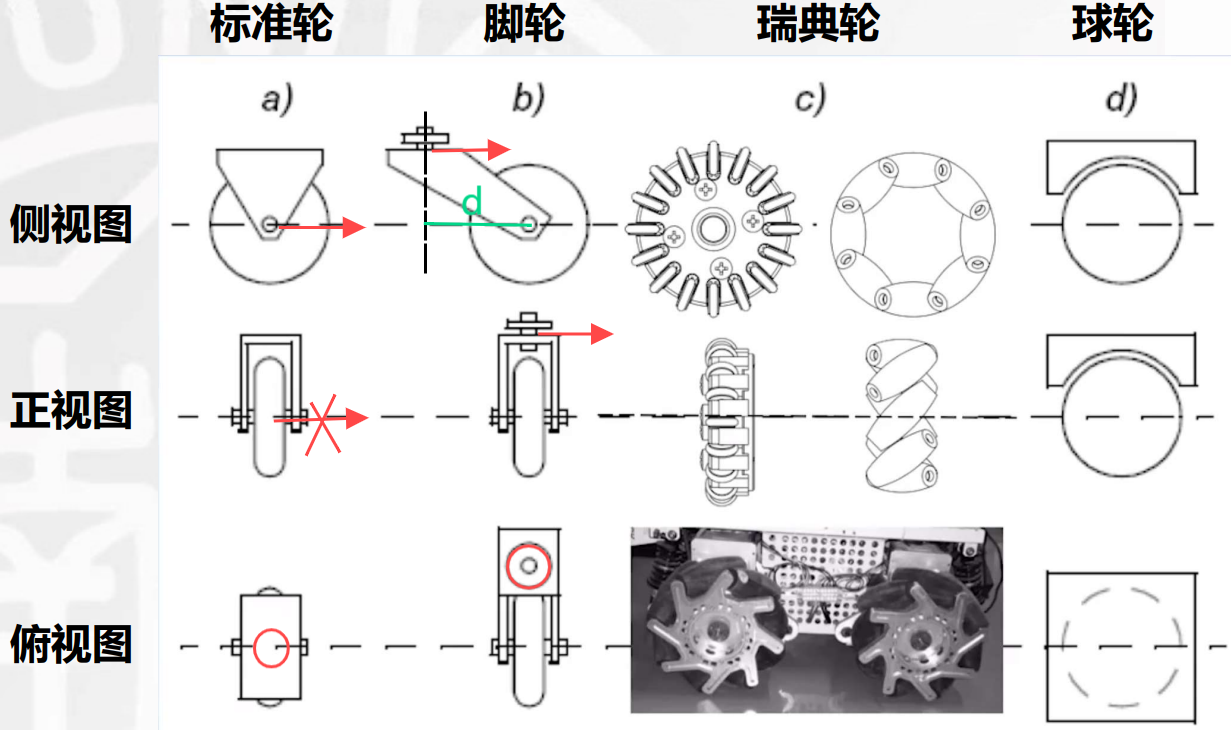
\includegraphics[width=0.7\textwidth]{tire} 
\caption[车轮类型]{车轮类型}
\end{figure}
%------------------------------------------------
\paragraph{标准轮(Standard wheel)}
\begin{itemize}
\item 两个自由度:沿轮平面滚动+沿垂直轴转动。 \\
一个约束:沿轮轴滑动。
\item 分类
\begin{itemize}
\item 标准固定轮:无法旋转,只有一个自由度。
\item 标准转向轮(舵轮)。
\end{itemize}
\end{itemize}
%------------------------------------------------
\paragraph{脚轮(Castor wheel)}
\begin{itemize}
\item 三个自由度:沿轮平面滚动+沿垂直轴转动+沿路轴运动。 \\
无约束。
\item 偏心距$ d $:触地点到垂直旋转轴距离。
\item 扭矩压力,易损坏。
\end{itemize}
%------------------------------------------------
\paragraph{瑞典轮(Swedish wheel)}
\begin{itemize}
\item 三个自由度:沿轮平面滚动(被动)+沿轮轴转动(主动)+沿垂直轴转动(被动)。 \\
无约束。
\item 麦克纳姆轮(Macanum wheel):45°,至少需要$ 4 $个共同使用。 \\
连续切换轮:90°,至少需要$ 3 $个共同使用。
\item 对地面冲击大,噪音大,易损坏,成本高。
\end{itemize}
%------------------------------------------------
\paragraph{球轮(Spherical wheel)}
\begin{itemize}
\item 三个自由度(全主动):沿两个正交轮轴转动+沿垂直轴转动。 \\
无约束。
\item 成本高,可靠性差。
\end{itemize}
%------------------------------------------------
\subsubsection{选取}
\begin{itemize}
\item 数量:至少三轮同时着地,才能保证静态稳定性。四轮可以提升稳定性,但需要适当的悬架系统。
\item 大小:越大的轮子通过性越好,但需要更大的扭矩。
\item 多数形态都有非完整约束。
\end{itemize}
%------------------------------------------------
\subsection{运动学建模}
%------------------------------------------------
\subsubsection{空间描述与状态表达}
%------------------------------------------------
\paragraph{坐标系}
\begin{itemize}
\item 惯性参考坐标系I:作业目标、控制指令、传感器感知测量信息。
\item 机器人参考坐标系R:控制器误差输入、控制器控制指令。
\item 笛卡尔坐标系:右手法则。
\end{itemize}
%------------------------------------------------
\paragraph{位姿(Pose)}~\\

位置空间求导得到速度空间:
$$
\xi_I = \begin{bmatrix} x_I \\ y_I \\ \theta_I \end{bmatrix}, 
\xi_R = \begin{bmatrix} x_R \\ y_R \\ \theta_R \end{bmatrix}
\overset{\text{求导}}{\Longrightarrow}
\xi_I = \begin{bmatrix} \dot{x}_I \\ \dot{y}_I \\ \dot{\theta}_I \end{bmatrix},
\xi_R = \begin{bmatrix} \dot{x}_R \\ \dot{y}_R \\ \dot{\theta}_R \end{bmatrix}
$$

惯性参考坐标系旋转得到机器人参考坐标系:
$$
\dot{\xi}_R = R\theta \dot{\xi}_I
$$

旋转阵
$ R(\theta) = \begin{bmatrix} \cos\theta & \sin\theta & 0 \\ -\sin\theta & \cos\theta & 0 \\ 0 & 0 & 1 \end{bmatrix} $
为单位正交阵,$ R^T = R^{-1} $。
%------------------------------------------------
\subsubsection{ICR法}\tip{ICR法运动学建模}
%------------------------------------------------
\paragraph{瞬时旋转/曲率中心(ICR)}
刚体上各点角速度相同。
\begin{figure}[H]
\centering 
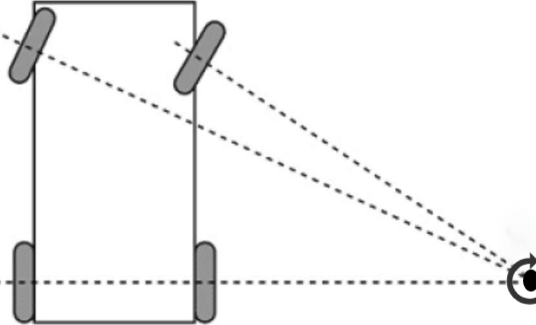
\includegraphics[width=0.4\textwidth]{icr_point} 
\caption[瞬心]{瞬心}
\end{figure}
%------------------------------------------------
\paragraph{步骤}
\begin{itemize}
\item 坐标系变换。
\item 确定约束。
\item 计算瞬心:各轮轮轴到该点距离与速度成正比。
\item 求解$ \xi_R = \begin{bmatrix} \dot{x}_R & \dot{y}_R & \dot{\theta}_R \end{bmatrix}^T $。
\end{itemize}
%------------------------------------------------
\subsubsection{约束方程法}\tip{约束方程法运动学建模}
%------------------------------------------------
\paragraph{要求}
在水平面上运动,车轮与地面点接触,不变形,安装在钢体表面,舵机转轴与地面垂直。
%------------------------------------------------
\paragraph{标准轮}
\begin{figure}[H]
\centering 
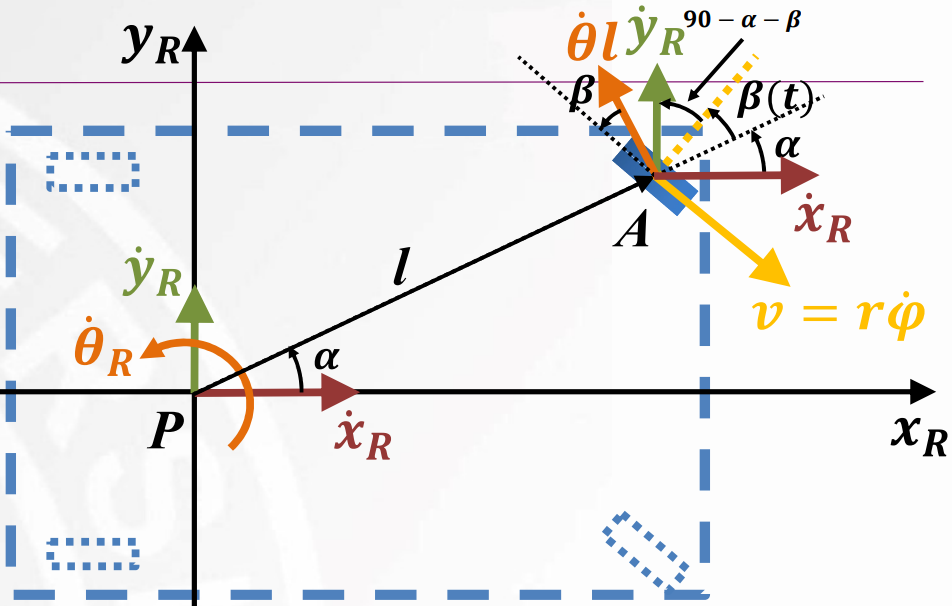
\includegraphics[width=0.6\textwidth]{Standard_wheel} 
\caption[标准轮约束方程]{标准轮约束方程}
\end{figure}

\begin{itemize}
\item 纯滚动:$ \begin{bmatrix} \sin(\alpha + \beta(t)) & -\cos(\alpha + \beta(t)) & -l\cos\beta(t) \end{bmatrix} R\theta \dot{\xi}_I = r\dot{\varphi} $。
\item 无滑动:$ \begin{bmatrix} \cos(\alpha + \beta(t)) & \sin(\alpha + \beta(t)) & l\sin\beta(t) \end{bmatrix} R\theta \dot{\xi}_I = 0 $。
\item 主动轮两个约束,随动轮只有滑动约束。
\end{itemize}
%------------------------------------------------
\paragraph{脚轮}
\begin{figure}[H]
\centering 
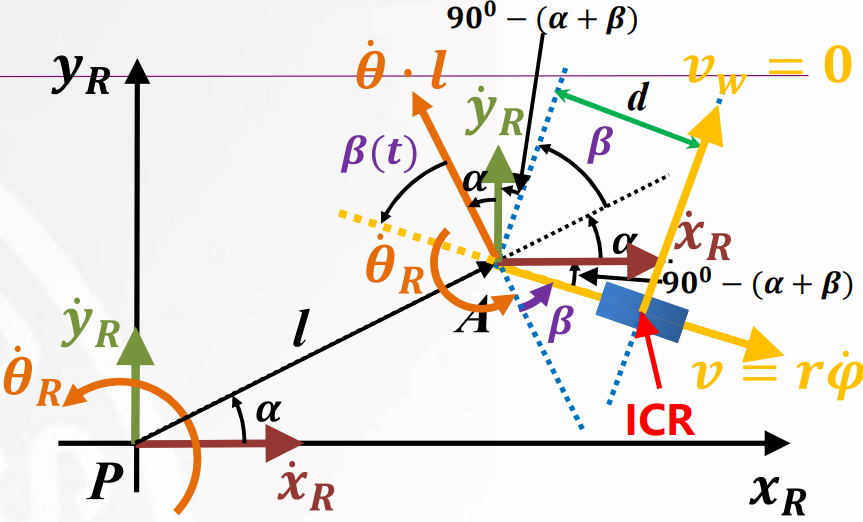
\includegraphics[width=0.6\textwidth]{Castor_wheel} 
\caption[脚轮约束方程]{脚轮约束方程}
\end{figure}

\begin{itemize}
\item 纯滚动:$ \begin{bmatrix} \sin(\alpha + \beta) & -\cos(\alpha + \beta) & -l\cos\beta \end{bmatrix} R\theta \dot{\xi}_I = r\dot{\varphi} $。
\item 无滑动:$ \begin{bmatrix} \cos(\alpha + \beta) & \sin(\alpha + \beta) & d + l\sin\beta \end{bmatrix} R\theta \dot{\xi}_I = -d\dot{\beta} $。
\item 主动轮两个约束,随动轮无约束。
\end{itemize}
%------------------------------------------------
\paragraph{瑞典轮}
\begin{figure}[H]
\centering 
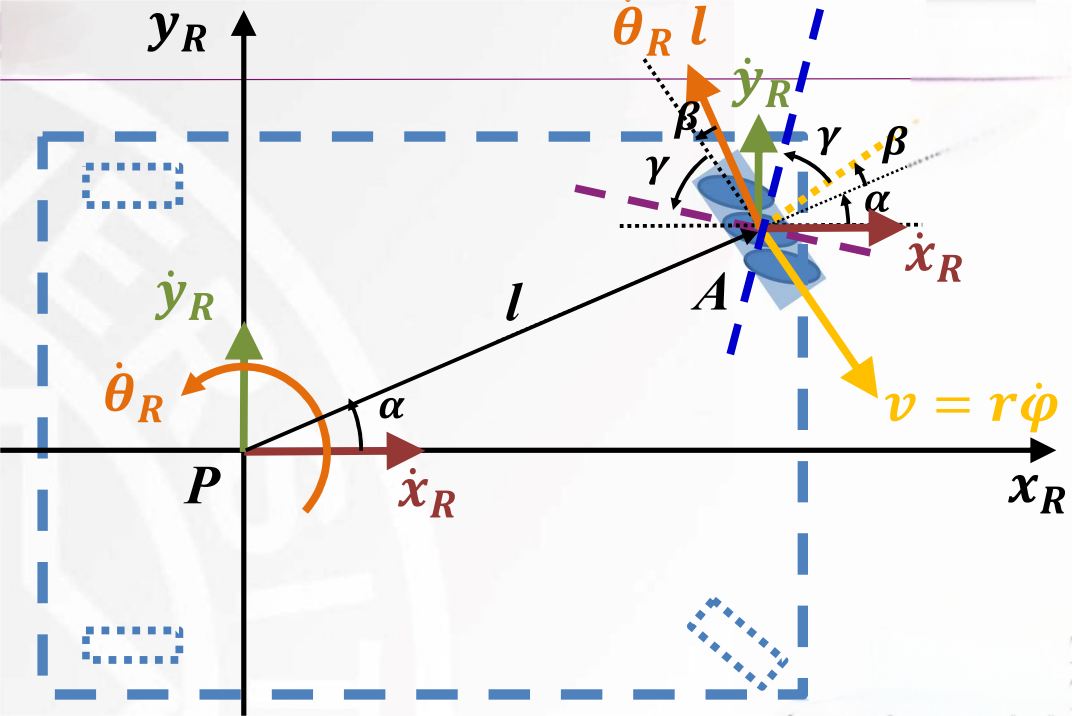
\includegraphics[width=0.6\textwidth]{Swedish_wheel} 
\caption[瑞典轮约束方程]{瑞典约束方程}
\end{figure}

\begin{itemize}
\item 纯滚动:$ \begin{bmatrix} \cos(\alpha + \beta + \gamma) & \sin(\alpha + \beta + \gamma) & l\sin(\beta + \gamma) \end{bmatrix} R\theta \dot{\xi}_I = r\dot{\varphi}\sin\gamma + r_{sw}\dot{\varphi}_{sw} $。
\item 无滑动:$ \begin{bmatrix} \sin(\alpha + \beta + \gamma) & -\cos(\alpha + \beta + \gamma) & -l\cos(\beta + \gamma) \end{bmatrix} R\theta \dot{\xi}_I = r\dot{\varphi}\cos\gamma $。
\item 需满足主动轮小轮两个约束,随动轮无约束。
\end{itemize}
%------------------------------------------------
\paragraph{使用}
根据各轮主/随动状态列运动约束方程,得到最多三个独立约束方程(对应平面的三维位姿)。

以下以$ N $个标准轮($ N_f $个固定,$ N_s $个转向)的机器人为例:
\begin{itemize}
\item 滚动约束
$$ J_1(\beta_s) R(\theta) \dot{\xi}_I - J_2 \dot{\varphi} = 0 $$

其中
$ 
J_1(\beta_s) =  \begin{bmatrix} {J_{1f}}_{(N_f \times 3)} \\ {J_{1s}(\beta_s)}_{(N_s \times 3)} \end{bmatrix},
\varphi(t) = \begin{bmatrix} \varphi_f(t) \\ \varphi_s(t) \end{bmatrix},
J_2 = diag(r_1, \cdots, r_N)\text{为轮径对角阵}
$。
\item 滑动约束
$$ C_1(\beta_s) R(\theta) \dot{\xi}_I = 0 $$

其中$ C_1(\beta_s) = \begin{bmatrix} {C_{1f}}_{(N_f \times 3)} \\ {C_{1s}(\beta_s)}_{(N_s \times 3)} \end{bmatrix} $。
\end{itemize}
%------------------------------------------------
\subsubsection{例子}\label{sec:example1}
以下以两轮差速机器人(见\ref{sec:two_wheel})为例,$ \alpha = \frac{\pi}{2}, \beta = 0 $:
\begin{figure}[H]
\centering
\subfloat[ICR法]{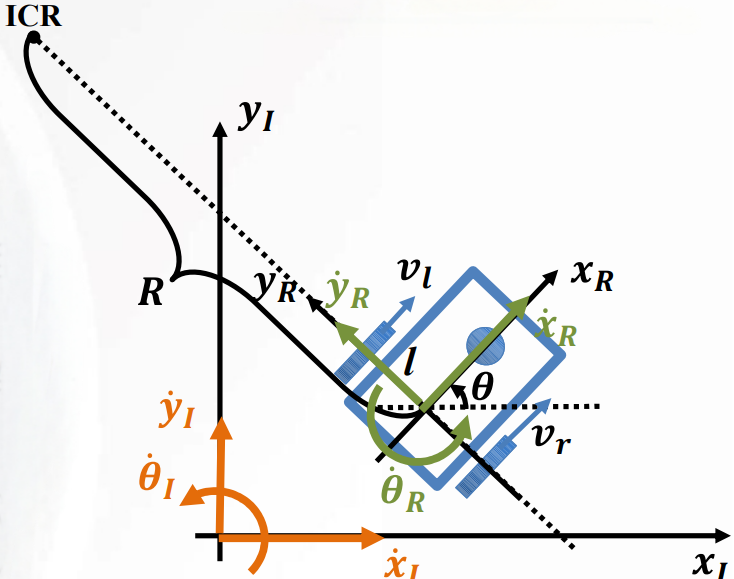
\includegraphics[width=.35\textwidth]{icr}} \quad
\subfloat[约束方程法]{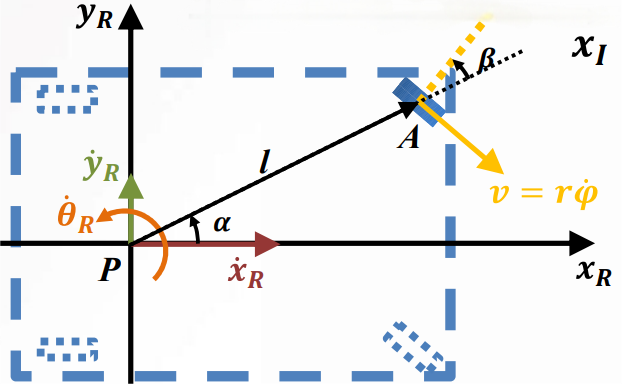
\includegraphics[width=.4\textwidth]{Equation_of_motion}}
\caption[两轮差速机器人正运动学建模]{两轮差速机器人正运动学建模}
\end{figure}
%------------------------------------------------
\paragraph{ICR法}~\\

两轮差速机器人的瞬心在两轮轮轴上,设其到机器人两轮中间的距离为$ R $,有:
$$ \dot{\theta} = \frac{\dot{x}_R}{R} = \frac{\dot{\varphi}_l r}{R-l} = \frac{\dot{\varphi}_r r}{R+l} $$

解得$ R = \frac{\dot{\varphi}_r + \dot{\varphi}_l}{\dot{\varphi}_r - \dot{\varphi}_l} $,代回即可。
%------------------------------------------------
\paragraph{约束方程法}
\begin{itemize}
\item 纯滚动:$ \begin{bmatrix} \sin(\alpha + \beta) & -\cos(\alpha + \beta) & -l\cos\beta \end{bmatrix} \dot{\xi}_R = r\dot{\varphi} $。
\item 无滑动:$ \begin{bmatrix} \cos(\alpha + \beta) & \sin(\alpha + \beta) & l\sin\beta \end{bmatrix} \dot{\xi}_R = 0 $。
\end{itemize}
%------------------------------------------------
\paragraph{正运动学模型}
$$ \dot{\xi}_R = \begin{bmatrix} \dot{x}_R \\ \dot{y}_R \\ \dot{\theta}_R \end{bmatrix} = \frac{r}{2} \begin{bmatrix} \dot{\varphi}_l + \dot{\varphi}_r \\ 0 \\ \frac{\dot{\varphi}_r - \dot{\varphi}_l}{l} \end{bmatrix} $$
%------------------------------------------------
\subsection{自由度}
%------------------------------------------------
\paragraph{概念}
\begin{itemize}
\item 衡量机器人改变运行状态的能力。
\item 需满足实际作业需求,考虑实现成本。
\item 机器人设计基础、算法依据(一般自由度相同的机器人可采用相同的控制和规划算法)。
\item 平面运动机器人自由度最大不能超过$ 3 $。
\end{itemize}
%------------------------------------------------
\paragraph{分类}\tip{自由度分类}
\begin{itemize}
\item 移动度(Degree of Mobility)$ \delta_m $:瞬时改变机器人运动状态的能力。
$$ \delta_m = \dim[C_1(\beta_s)] = 3 - \operatorname{rank}[C_1(\beta_s)] \in [0,3] $$
\item 转向度(Degree of Steerability)$ \delta_s $:间接改变机器人运动状态的能力。
$$ \delta_s = \operatorname{rank}[C_{1s}(\beta_s)] \in [0,2] $$
\item 机动度(Degree of Maneuverability)$ \delta_M $:改变机器人运动状态的能力。
$$ \delta_M = \delta_m + \delta_s $$
\begin{itemize}
\item 机动度相同,结构不一定相同。
\item $ \delta_M = 2 $,瞬心位于一条直线上;$ \delta_M = 3 $,瞬心可分布于空间任何一点。
\end{itemize}
\end{itemize}
%------------------------------------------------
\paragraph{实例}
\begin{itemize}
\item 全向机器人:
\begin{itemize}
\item Type(3,0):完整约束全方位移动机器人。
\item Type(2,1):一个同心轮+两个瑞典轮。
\item Type(1,2):多舵机全方位移动机器人。
\end{itemize}
\item 非全向机器人:
\begin{itemize}
\item Type(2,0):差分移动机器人。
\item Type(1,1):自动驾驶汽车(阿克曼转向)、自行车、叉车。
\end{itemize}
\end{itemize}
%----------------------------------------------------------------------------------------
\section{机器人运动控制}
%------------------------------------------------
\subsection{定点控制器}
%------------------------------------------------
\subsection{轨迹跟踪控制器}
%------------------------------------------------
\subsection{路径跟踪控制器}
%----------------------------------------------------------------------------------------
\section{机器人感知}
%------------------------------------------------
\subsection{传感器}
%------------------------------------------------
\subsection{激光定位}
%------------------------------------------------
\subsection{SVD与ICP}
%------------------------------------------------
\subsection{卡尔曼滤波}
%------------------------------------------------
\subsection{蒙特卡洛定位}
%------------------------------------------------
\subsection{SLAM}
%----------------------------------------------------------------------------------------
\section{机器人轨迹规划}
%----------------------------------------------------------------------------------------
\section{数理补充}
%----------------------------------------------------------------------------------------
\end{document}